\documentclass[a4paper, 12pt, titlepage]{article}

% Document quality things
\usepackage[utf8]{inputenc}
\usepackage{microtype, xcolor}
\usepackage{csquotes}
\usepackage{url, hyperref}
\hypersetup{colorlinks=true, linkcolor=black, citecolor=black, urlcolor=blue}

% Image-related packages
\usepackage{graphicx}
%\usepackage{float}
\graphicspath{{./gfx/}}
%\usepackage[font=small,skip=5pt]{caption}

% Setting margins
\usepackage[a4paper,bottom=2cm,top=2cm,left=2.5cm,right=2.5cm, includefoot]{geometry}

% Table helper packages
%\usepackage{multirow, multicol}
%\usepackage{makecell}
%\usepackage{array}
%\usepackage{tabularx} % Not needed currently, but has a few nice options
%\usepackage{wrapfig} % Floating figures/tables
\usepackage{booktabs}
\usepackage{longtable}

% Prevents spamming tedious newlines everywhere, also disables auto indentation, etc.
\usepackage[skip=0.75\baselineskip plus 2pt]{parskip}

% Self-explanatory
%\usepackage{titlesec}
%\titleformat{\section}[block]{\normalfont\scshape\Large}{\thesection}{1em}{}
%\titleformat{\subsection}{\normalfont\large}{\thesubsection}{1em}{}

\title{
    {CS 319 - Object Oriented Software Engineering}\\
    {\small Instructor: Eray Tüzün, TA: Muhammad Umair Ahmed \& Elgun Jabrayilzade}\\
    {\vspace{10mm}BilHealth}\\
    {\Large \textbf{Design Report}}\\
    {\small Iteration 1}\\
    {\vspace{10mm}
\includegraphics[width=0.3\linewidth]{bilkentlogo}}
}
\author{
  Mehmet Alper Çetin\\ \texttt{21902324}
  \and
  Vedat Eren Arıcan\\ \texttt{22002643}
  \and
  Uygar Onat Erol\\ \texttt{21901908}
  \and
  Recep Uysal\\ \texttt{21803637}
  \and
  Efe Erkan\\ \texttt{21902248}
}
\date{\today}

% \usepackage{tikz}
% \usetikzlibrary{automata, positioning, arrows}

\usepackage{pdflscape, pdfpages}

\begin{document}
  \maketitle
  \tableofcontents
  \pagebreak

  \section{Introduction}

  Our project is a health center management software, built in the form a web application.
  This report documents the design choices that were made for the implementation of the project.

  Note that all diagrams on this document are in vector format, meaning that you can zoom in without any decrease in quality.

  \subsection{Purpose of the System}

  The project is designed as a web-based application that will ease the health center management in Bilkent.
  The main goal of the project is to provide online attention to the patients
  and to have better communication betweeen doctors, staff and patients.
  Our system includes features that ease the interaction betweeen patients and doctors through cases
  which contain all relevant information for a given medical situation.
  Patients can open cases and request for appointments through that opened cases.
  Also, staff and doctors provide patients with medical services through cases.

  \subsection{Design Goals}

  \subsubsection{Usability}

  The system should be easily usable by all actors to achieve its goal.
  We want to design a user interface such that a person who isn't familiar with using
  computers can easily find their way around the website.
  All the buttons and labels in the system will have self-explanatory titles and
  the system includes boundary conditions which prevent the user from doing something wrong,
  to increase the usability of the system.

  \subsubsection{Security}

  The system will have a person's health details which are highly privacy sensitive.
  Also, the system will have confidential information of every user such as Bilkent ID,
  email address and password. Therefore, the system should be secure to protect
  all of these personal information from any unauthorized activity.
  No user would want such private data to be accessed by any unauthorized person.

  \subsubsection{Maintainability}

  The system will be designed following a object-oriented programming model.
  This will ease making updates on different parts without harming to other parts.
  It also gives the opportunity to add new parts without changing all parts of the project.

  \subsubsection{Performance}

  The system should give the best performance even on computers with old hardware.
  Every user interaction should be processed and displayed in less than 1 second to provide
  a better experience to the user.

  \subsubsection{Scalability}

  The system aims to support up to 20 thousand users, which means the design should enable concurrency and high throughput.

  \subsubsection{Deployment}

  In order to facilitate the development of the project in a fast paced environment,
  the design takes into consideration concepts such as portability and replicability.
  The sought result is that developers can easily run a local version of the system while
  keeping things simple when the time comes to deploy to production.

  \subsubsection{Testability}

  Almost any respectable web service of today strives to achieve test driven development of some magnitude.
  Our project is no different and the design attempts to make it possible to incorporate unit or integration tests
  for the business logic, by means such as dependency injection.

  \subsubsection{Extensibility and Maintainability}

  The fast paced development environment can quickly turn the project into a nightmare of spaghetti code and architecture.
  To counteract such a possibility, the design aims to keep components maintainable and extensible through proven OOP structs.

  \section{High-Level Software Architecture}

  \subsection{Subsystem Decomposition}

  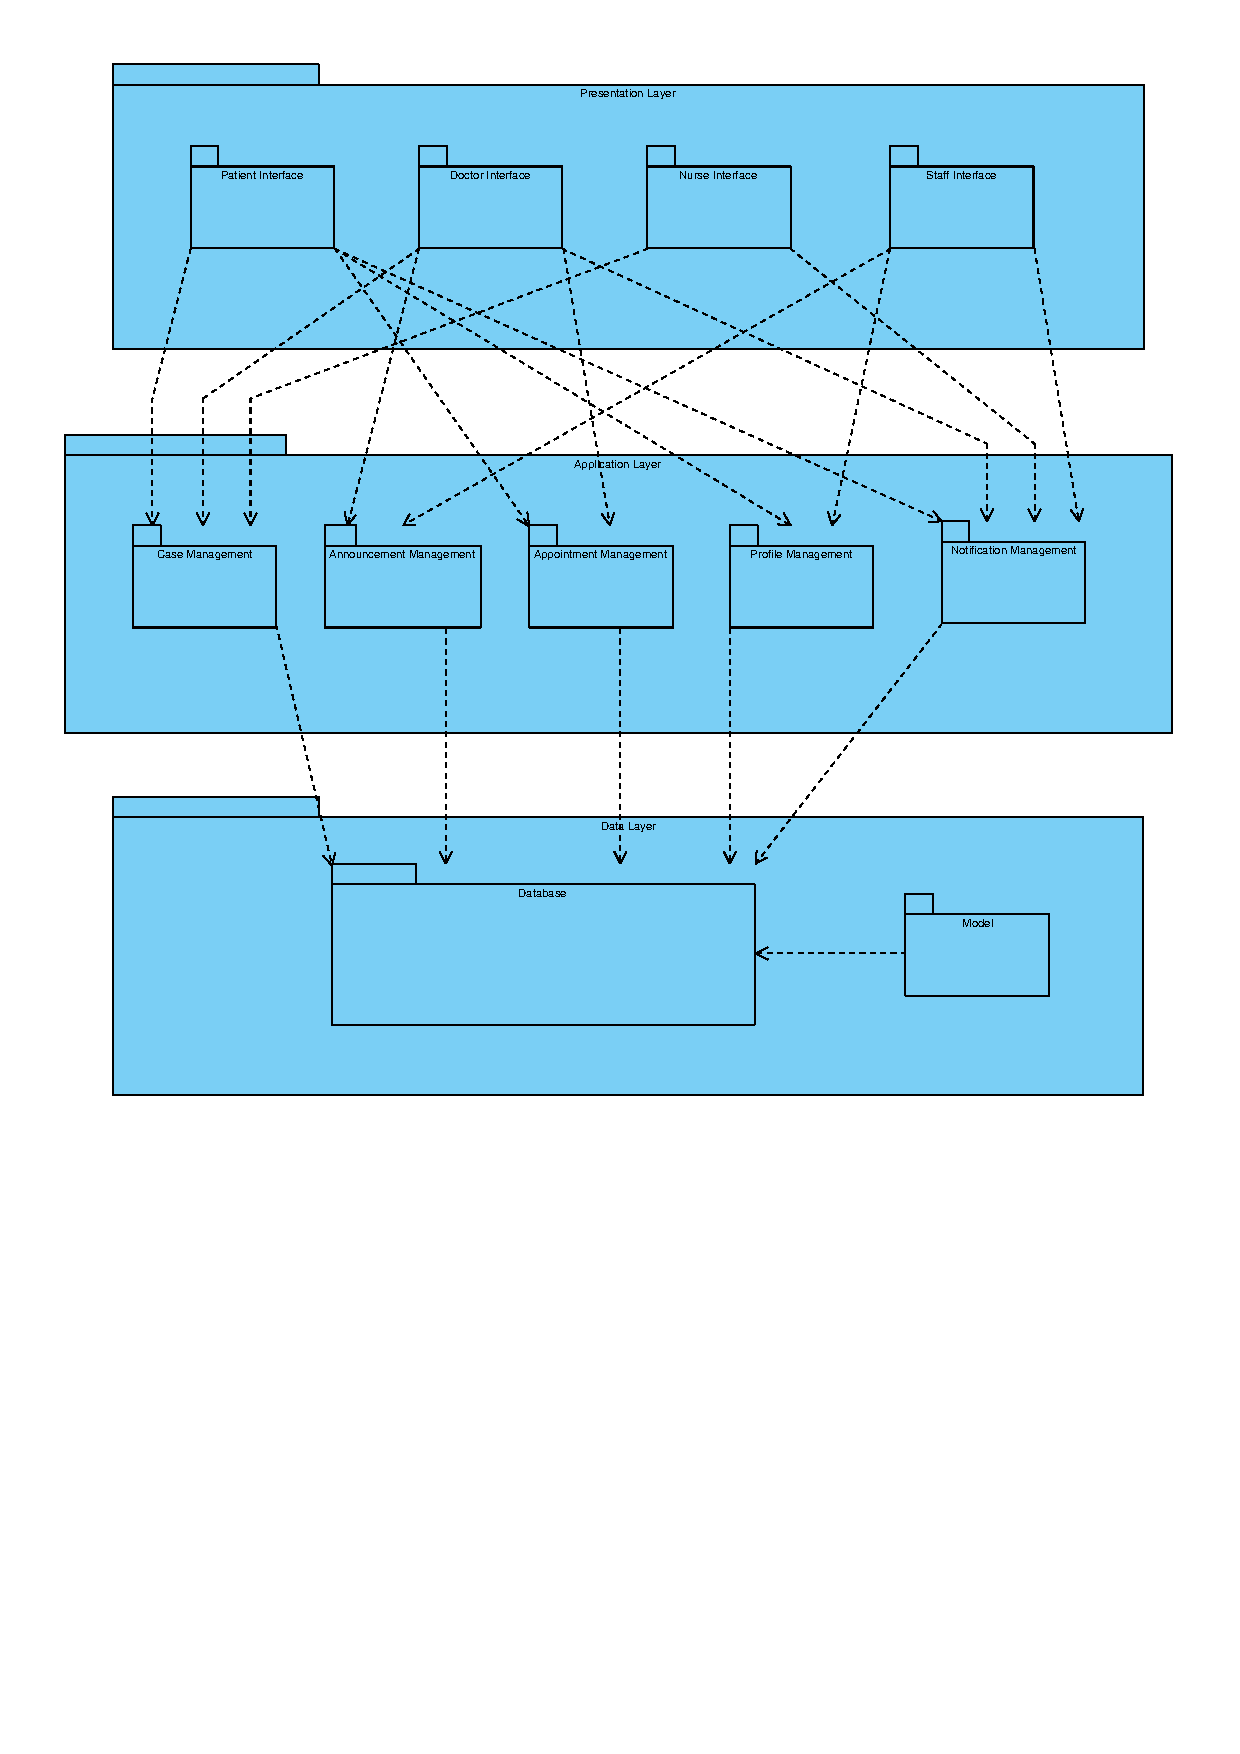
\includegraphics[width=\linewidth]{subsystem}

  \subsection{Hardware-Software Mapping}

  The project does not have any extraordinary hardware requirements.
  As it is a web application, it requires the users to have a device using which they can
  connect to the web server of the application over the internet.
  The main target devices for a supported user experience are desktop computers, laptops, and mobile phones.

  In order to run the project the intended way, the host system's hardware must support stable containerization through Docker.
  It is possible to reconfigure certain entrypoints of the project to support bare-metal execution too, at the cost of
  system replicability and practicality.
  Similar to most other web services, the project is officially supported to run on a Linux environment, which
  may be of consideration when choosing hardware.

  \subsection{Persistent Data Management}

  The project makes use of PostgreSQL as its persistent data storage solution.
  The project does not have specific requirements that directly justify the use of PostgreSQL,
  however, this database system is well rounded enough to save the development process from any potential drawbacks.
  The \texttt{psql} command line tool is easy to use and supports our workflow in implementing database migrations.
  Also, the Docker images for the database are robust and simple,
  which has allowed the project to be supported by a containerized database.

  On top of the actual database, the project uses EF Core as an object relational mapper (ORM),
  which is Microsoft's official library for data persistence.
  We use the recommended \textit{code-first} approach of database management, which means our PostgreSQL tables are
  constructed by EF Core with respect to our entity definitions in C\# code.
  The EF Core toolchain generates migrations, which it also converts to SQL scripts,
  using which a database can be configured to host the project in moments.

  \subsection{Access Control and Security}

  The project is secured by a typical authentication and authorization flow,
  supported by our identity provider of choice, ASP.NET Core Identity.
  Authentication is conducted over HTTPS with a user's username and password.
  The controller endpoints of the project are exposed to users within specific role types,
  which constitutes our authorization process.
  The authentication is persisted on the user's device in the form of browser cookies, enabling user session capability.

  The project is mostly exclusive to authenticated users, meaning that there are not many substantial actions a guest user can take.
  Moreover, since users are divided across roughly 5 roles,
  most HTTP endpoints concerning management of the system are forbidden to access by non-staff users.

  Lastly, user details are stored in a database with their passwords having been hashed by the \textit{bcrypt} algorithm,
  which is among the top choices in secure password storage techniques at this time.

  \subsection{Boundary Conditions}

  \subsubsection{Initialization}

  The project is a web application and does not require any initialization.
  The access is easy through the web.
  To access the website, only an internet connection is required.
  Since the website is not protected, there are no extra requirements in this regard.
  Once accessed, an account is needed for further actions.
  To login, one needs a Bilkent ID and permission from the admins of the project.

  \subsubsection{Termination}

  Since the project is a web application, ending the process is enough to terminate the application.
  Through maintenances, the application will be terminated by admins and no users will be able to use the website.
  Since the application is for the health center, the maintenance sessions will be no longer than 30 minutes each week.

  \subsubsection{Failure}

  Being a website the most noxius failure is DDoS attacks.
  DDoS attacks are on availability of the server and as a health center application we should guarantee that users does not have
  any trouble using the website.
  We will use Web Application Firewall (WAF) against these attacks to make sure our site does not go down.

  \section{Low-Level Design}

  \subsection{Object Design Trade-Offs}

  \begin{itemize}
    \item \textbf{Maintainability} versus \textbf{Performance:}
      The system will have objects for almost every part of the project because it is coded using OOP.
      This situation will cause a decrease in performance but it is good for maintainability
      because it provides developers the option to make changes easily.
    \item \textbf{Memory} versus \textbf{Performance:}
      The system will be created using OOP, so there will be lots of objects and classes
      for almost every part of the project.
      This causes a lot of memory usage but it can be handled by AWS which lowers the memory usage.
      It increases the memory optimization and performance.
    \item \textbf{Security} versus \textbf{Usability:}
      The system will not have two way authentication for accounts.
      In other words, user can access his/her account with only password.
      This can be cause a problem for security but it increases the usability of the system.
    \item \textbf{Functionality} versus \textbf{Usability:}
      The project system will be used by patients, staff, doctors and nurses.
      This forces the project to have many functionalities which are not available for everyone.
      This decreases the usability.
  \end{itemize}

  \subsection{Final Object Design}

  \subsection{Packages}

  Below is a list of our namespaces with brief descriptions.
  Note that, to preserve the anonimity of the report, we've replaced the root namespace with a placeholder ``\texttt{Project}''.

  \begin{itemize}
    \item \texttt{Project.Utility}\textbf{:}\\
      This namespace contains the utility functions which were able to be decoupled from the project at large.
      In doing so, it can be used reliably across other namespaces.
    \item \texttt{Project.Utility.Enum}\textbf{:}\\
      This namespace contains the \textit{enum} and \textit{enum class} definitions that are used in many parts of the project.
    \item \texttt{Project.Services}\textbf{:}\\
      This namespace contains the main business logic interface through which boundary and entity systems are connected.
    \item \texttt{Project.Services.Users}\textbf{:}\\
      This namespace carries the same responsibility as its parent, but specifically for user-related entities.
    \item \texttt{Project.Model}\textbf{:}\\
      This namespace contains the entities that are persisted into a database. The main units of data are located here.
    \item \texttt{Project.Model.Identity}\textbf{:}\\
      This namespace contains entities that are specifically user information holding objects.
    \item \texttt{Project.Model.Dto}\textbf{:}\\
      This namespace contains \textit{record} objects that are used to transfer data to and from the front-facing controllers.
      It is also used for some internal communication of unpersisted data.
      In other words, these are temporary representations of the actual data entities to be persisted.
    \item \texttt{Project.Data}\textbf{:}\\
      This namespace contains the database context built from EF Core's repository-like architecture.
    \item \texttt{Project.Controllers}\textbf{:}\\
      This namespace contains the front-facing API endpoints through which external communication with clients take place.
  \end{itemize}

  \subsubsection{External Packages}

  \begin{itemize}
    \item \texttt{Microsoft.AspNetCore}\textbf{:}\\
      This package is the framework supporting the entire web application.
    \item \texttt{Microsoft.EntityFrameworkCore.Design}\textbf{:}\\
      This package allows the EF Core migration tool to work on the project.
    \item \texttt{Microsoft.AspNetCore.Diagnostics.EntityFrameworkCore}\textbf{:}\\
      This package allows debugging EF Core migrations.
    \item \texttt{npgsql.EntityFrameworkCore.PostgreSQL}\textbf{:}\\
      This package is the database driver providing EF Core its interoperation with PostgreSQL.
    \item \texttt{Microsoft.AspNetCore.Identity.EntityFrameworkCore}\textbf{:}\\
      This package provides authentication and authorization of users through integration with EF Core.
    \item \texttt{BCrypt.Net-Next}\textbf{:}\\
      This package provides the \textit{bcrypt} algorithm which is currently among the best in securely hashing user passwords.
    \item \texttt{Microsoft.AspNetCore.Mvc.NewtonsoftJson}\textbf{:}\\
      This package is the most popular JSON library for .NET, used as the default solution in most cases.
    \item \texttt{Microsoft.AspNetCore.SpaProxy}\textbf{:}\\
      This package allows the .NET build process to launch and proxy with the client application.
  \end{itemize}

  \subsection{Class Diagrams of Layers}

  \subsubsection{Data Access Layer}

  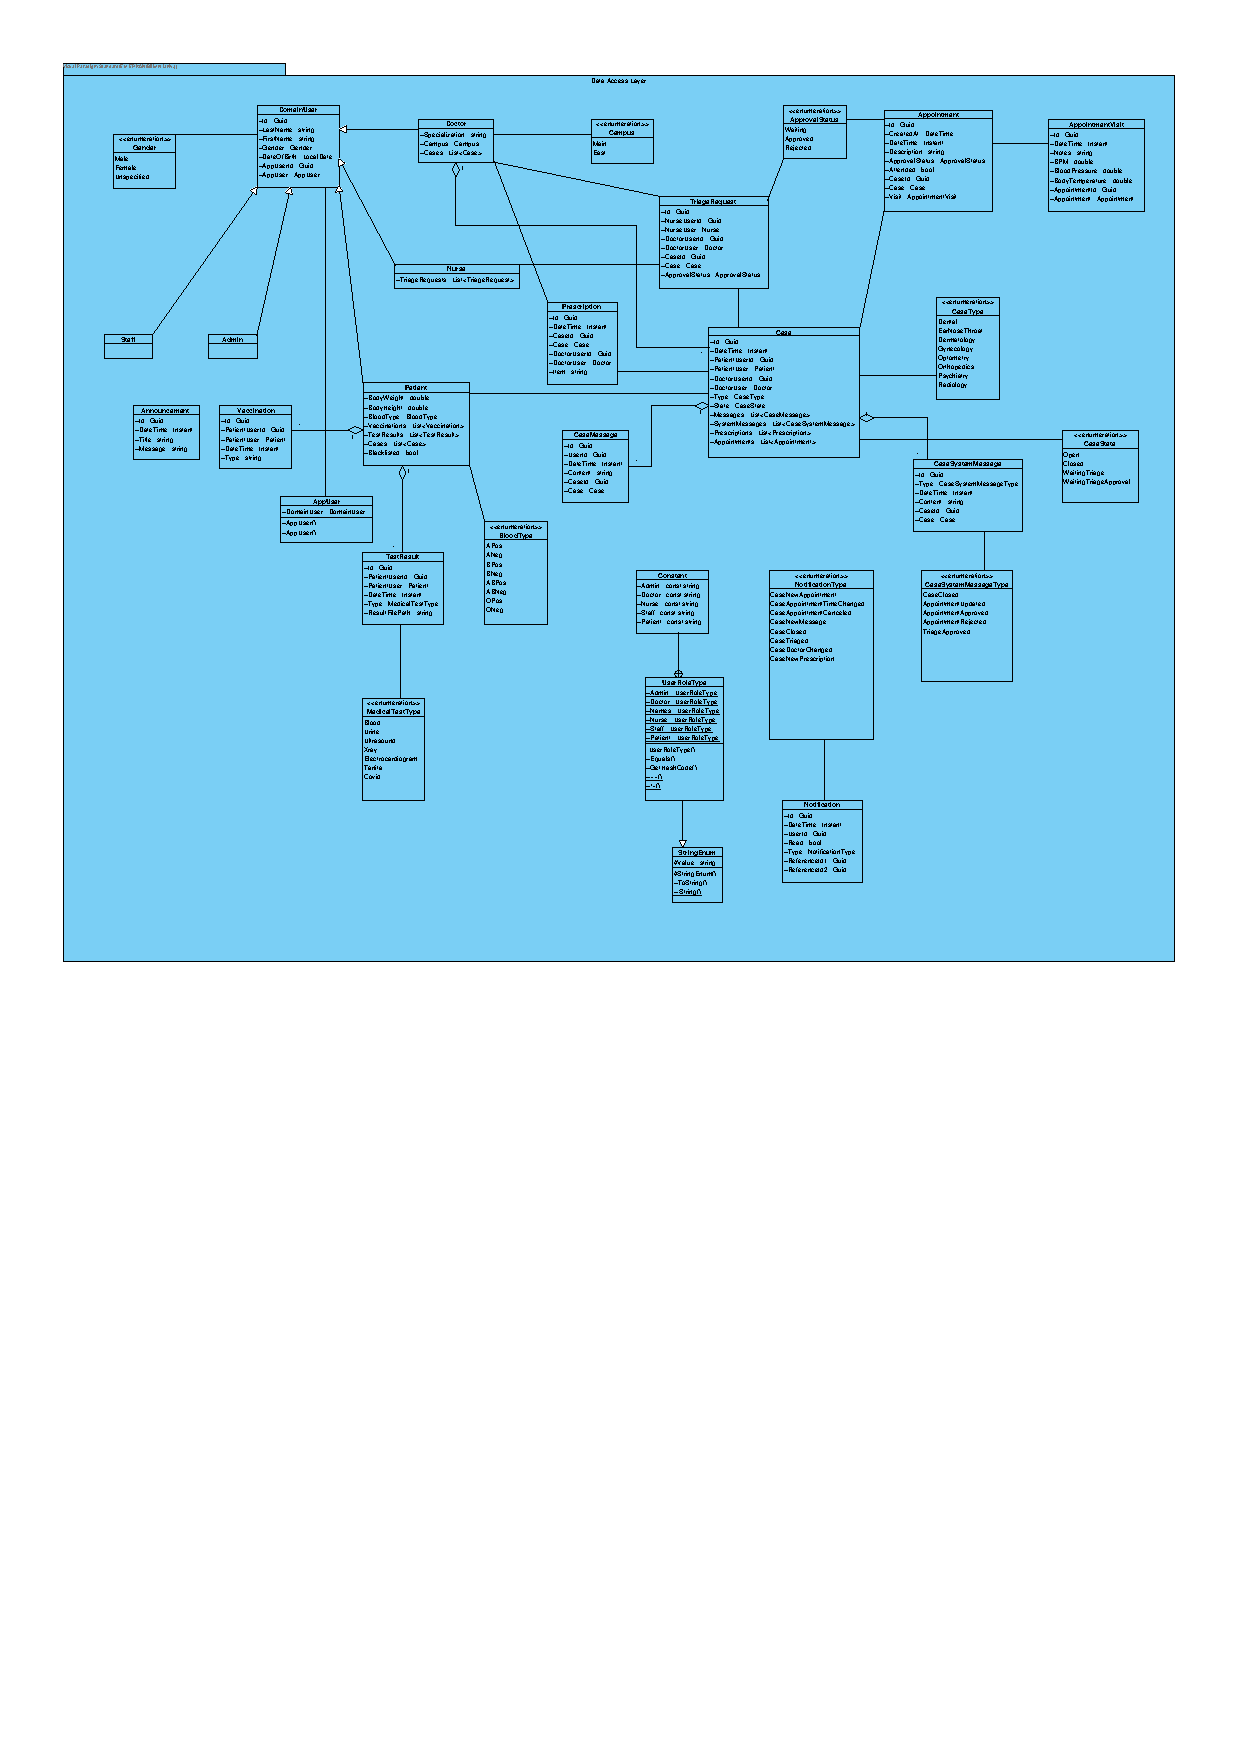
\includegraphics[width=\linewidth]{dataaccess}

  \subsubsection{Business Logic Layer}

  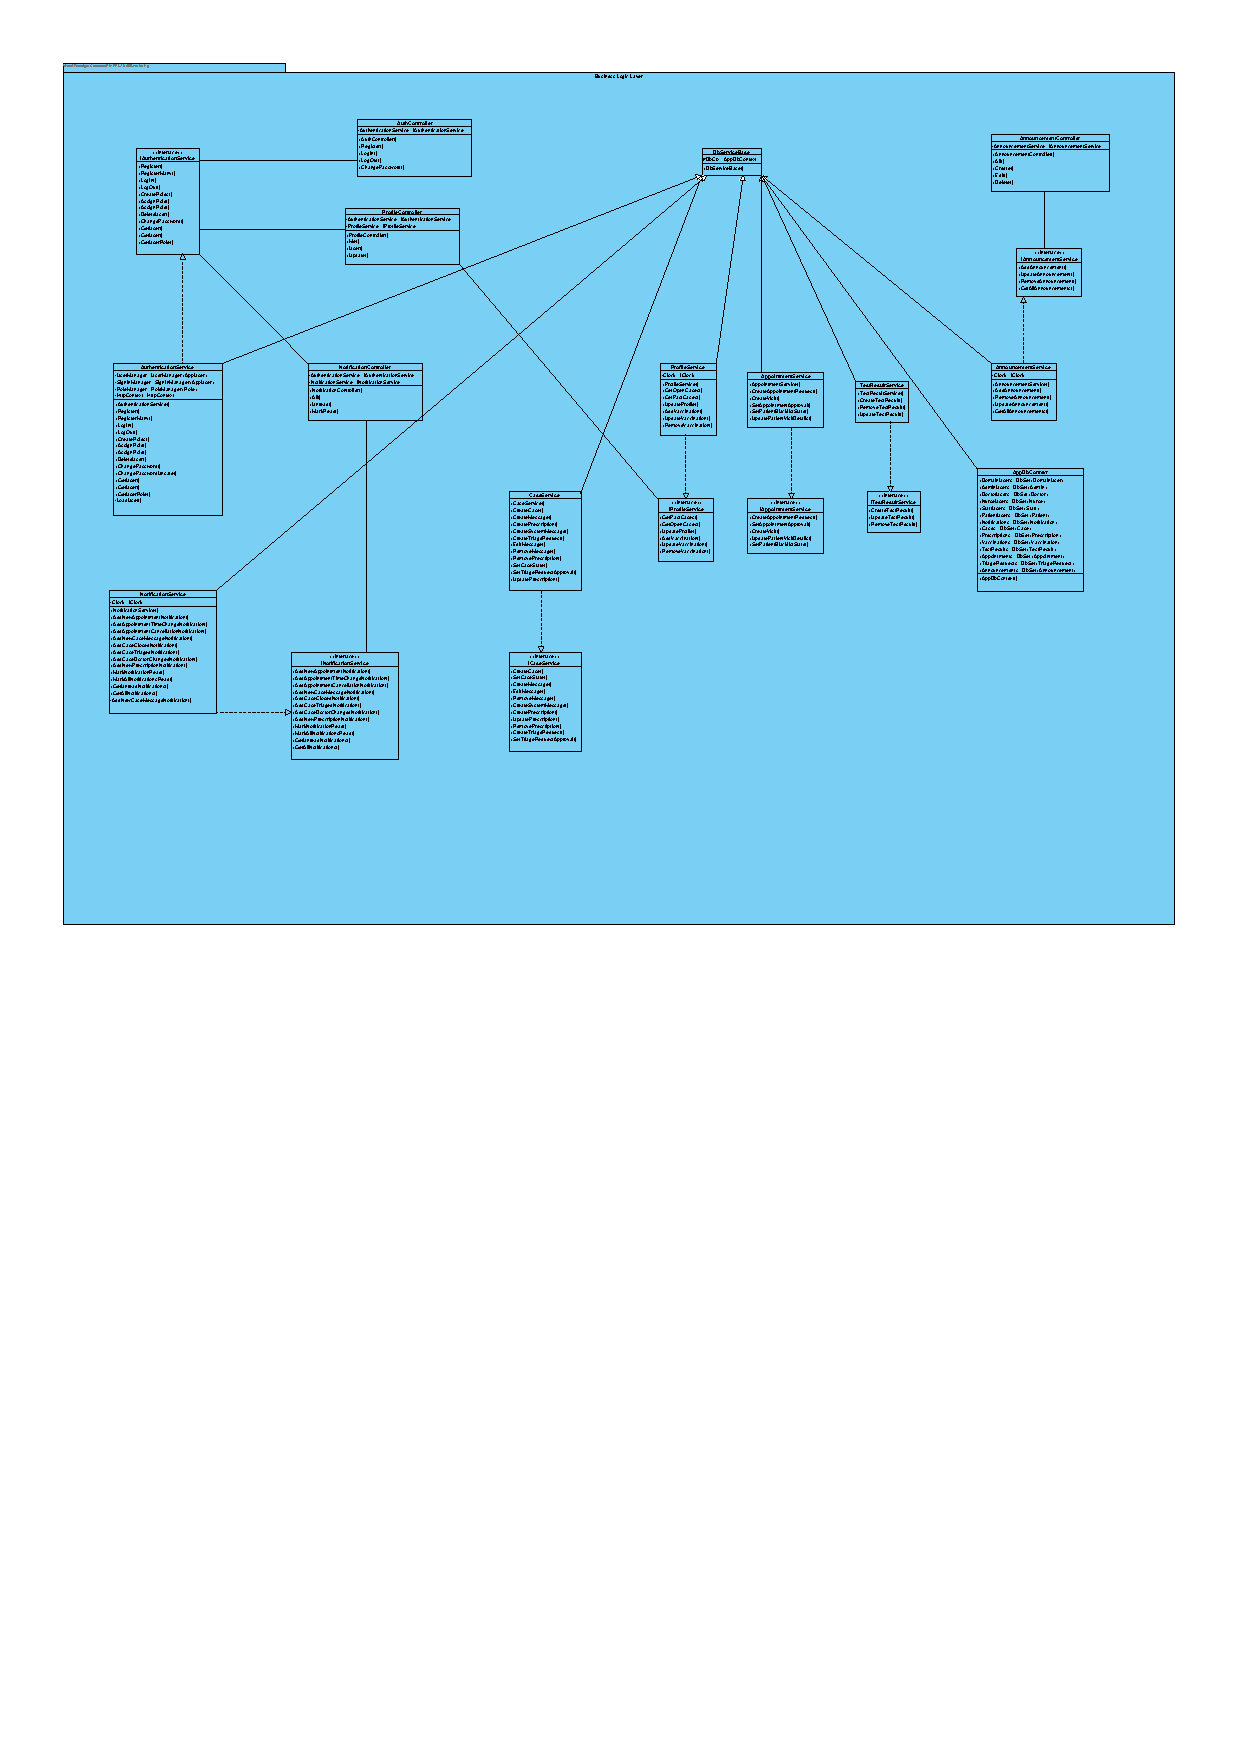
\includegraphics[width=\linewidth]{businesslogic}

  \subsubsection{User Interface Layer}

  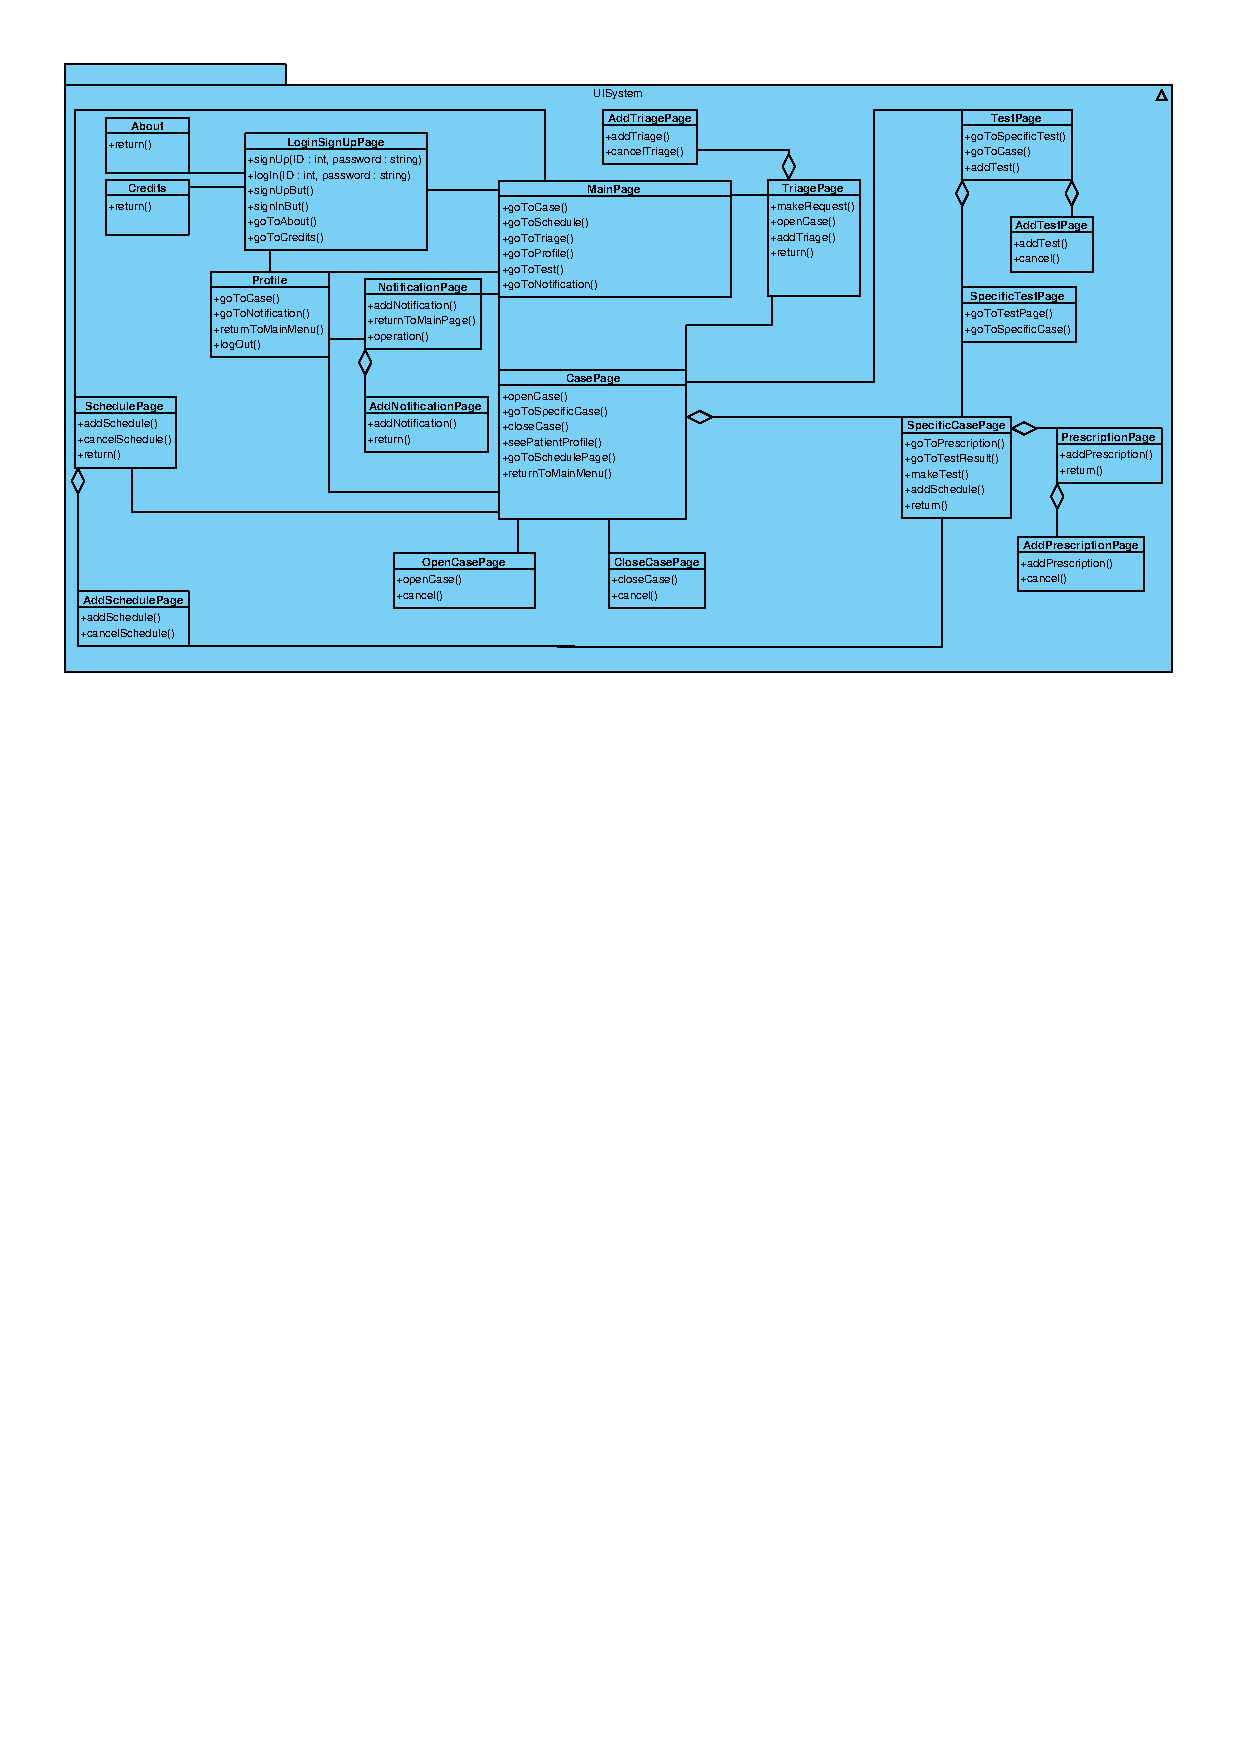
\includegraphics[width=\linewidth]{uisystem}

  \pagebreak
  \section{Glossary}

  \begin{itemize}
    \item \textbf{EF Core:} Microsoft's object relational mapper solution.
    \item \textbf{ORM:} Abbreviation for \textbf{O}bject \textbf{R}elational \textbf{M}apper.
    \item \textbf{.NET:} Microsoft's giant framework for C\# applications.
    \item \textbf{ASP.NET:} Microsoft's giant framework for web-based C\# applications.
    \item \textbf{PostgreSQL:} A popular relational database management system.
    \item \textbf{JSON:} Abbreviation for \textbf{J}ava\textbf{S}cript \textbf{O}bject \textbf{N}otation.
    \item \textbf{Hashing Passwords:} Cryptographically obscuring passwords such that they are practically irrecoverable.
    \item \textbf{Repository:} A very popular design pattern to provide an abstraction to persistent data.
    \item \textbf{API Endpoint:} The application programming interface endpoint through which communication with the system can occur.
    \item \textbf{Application Entrypoint:} The sum of the build process and configuration of the initialization of the system.
    \item \textbf{HTTP:} The most commonly used protocol over which web servers and clients communicate.
    \item \textbf{HTTPS:} Wraps the HTTP protocol into a cryptographically secured transmission protocol.
    \item \textbf{Enum:} A special type of programming entity that can be used to enumerate hard-coded types, mostly mapped to integers.
    \item \textbf{Enum Class:} An enum-like class adding specialized capability to the enum concept.
    \item \textbf{Record:} A C\# reference type with value-based equality.
    \item \textbf{Docker:} A software virtualization product.
    \item \textbf{Dependency Injection:} A software design pattern that inverses the dependency control by injecting dependencies into a dependent object.
  \end{itemize}

\end{document}
